\chapter{Heuristic algorithms}
\label{chapter5}

Heuristic algorithms are approaches designed for solving a given problem in a faster and more efficient fashion than traditional methods by trading optimality, accuracy, precision, or completeness for speed \cite{HeuristicsDefinition}. Are often used to solve problems where there is no known efficient way to find a solution quickly and accurately once they have low time complexity \cite{HeuristicsDefinition}. Also they are able to produce a solution individually or to be used to provide a good baseline when supplemented with optimization algorithms \cite{articleHeuristics}. There are many commonly used heuristics such as genetic algorithms, artificial neural networks and support vector machines \cite{HeuristicsDefinition}. When networks are too large, the dimensioning problem becomes too complex and so the ILP models can be very slow to obtain the solution, whereas heuristic solutions lead to good performances in practical network scenarios when presented a sufficiently feasible solution, instead of an optimal solution. Therefore, this chapter is organized in five subsections where some heuristic algorithms are proposed with a final major objective of minimizing the total CAPEX of a network. In subsection \ref{scheduling2} some sorting methods are approached, in subsection \ref{logicaltopology2} is addressed the conversion from the physical to the logical topology of a network and the respective implications, in subsection \ref{routing2} various routing strategies are debated and an explanation is given over the chosen method and in subsection \ref{G} the grooming strategy utilized is explained. Finally, in subsection \ref{WA} the possible wavelength assignment methods are discussed as well as some of the implications. The created algorithms in this dissertation were all developed in C++ language with the aid of Visual Studio IDE and some of the pseudo code developed for these algorithms is also shown below into various flowcharts which use rounded rectangle shapes to symbolize the beginning or the end of the program, parallelogram shapes to indicate a point where there is an input to the program, diamond shapes symbolizing decision points and rectangle shapes representing a whole variety of processes, such as, a simple assignment of a value to a variable, constant or parameter.

\section{Scheduling}
\label{scheduling2}

\begin{figure}[H]
  \begin{center}
    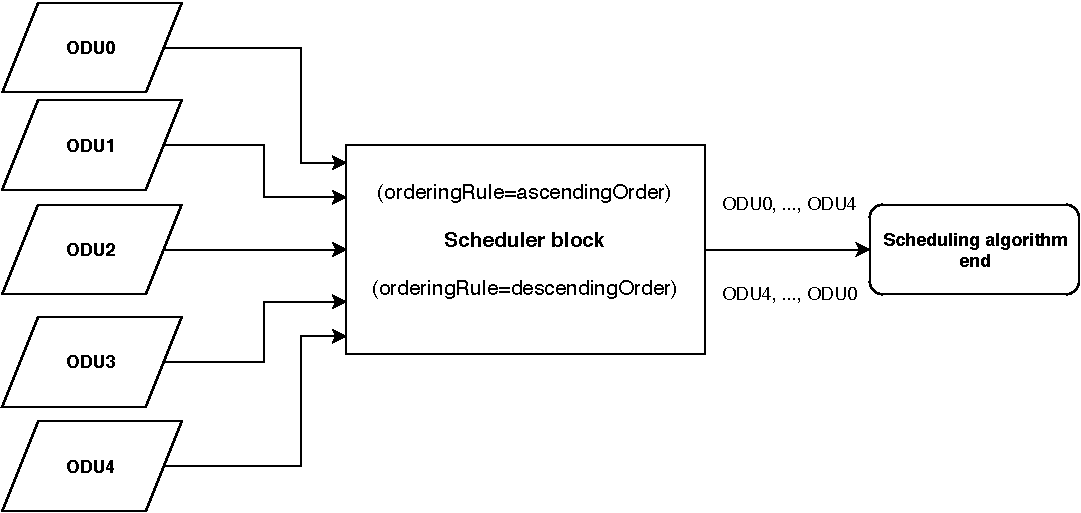
\includegraphics[width=0.9\textwidth]{fig/logos/schedulerAscending.pdf}
    \caption{Scheduler algorithm illustration considering both ordering rules.}
  \end{center}
  \label{schedulerAscending}
\end{figure}

\begin{figure}[H]
  \begin{center}
    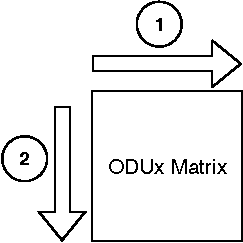
\includegraphics[width=0.3\textwidth]{fig/logos/scheduler2.pdf}
    \caption{Illustration of the order by which an ODUx traffic matrix is searched through.}
    \label{scheduler2}
  \end{center}
\end{figure}

There are many different possible strategies that can be used for traffic ordering purposes. Most may rely individually on the quantity of traffic of each request, the traffic granularity, the length of the shortest logical or physical paths either in terms of distance or hops, the need of protection paths, the quality of the path set in terms of desirable path options or a smart combination of some of this aspects \cite{SimmonsJane2008}. Other ordering strategies are also possible and in general none of them reclaims the best results for every practical scenario. In this specific scenario, as it is shown above in figure \ref{schedulerAscending} by choosing an ascending ordering rule the first demands to be processed will be of the ODU0 type, followed by ODU1, ODU2, ODU3 and finally ODU4. If on the other hand, it is chosen the descending ordering rule then demands will be processed in the backwards order. The chosen criteria for test performing purposes was the descending ordering rule since demands that require bigger bandwidths become harder to accommodate and thus should be the first ones to be processed in order to guarantee the assignment of the optimal paths.  Additionally, the way that each of the ODU demand matrices are searched through can be seen in figure \ref{scheduler2}, from left to right the demands originating in node one are the firsts to be processed and so on to the last node of the network. It is assumed that although multiple demands can be added at once till the network, each demand is processed individually before moving on to the next.
%The signal exiting from this block will be of the "Demand Request" type and will contain information of each demand's index, source and destination nodes, ODU type and survivability method chosen, if any. This signal is then sent to the logical topology manager. 
 
\section{Logical Topology}
\label{logicaltopology2}

As in this dissertation only the transparent transport mode is considered, then the logical and physical topologies will differ from each other since the first one will be a full mesh network \cite{Vasco}. Below in figure \ref{logicalAlgorithm} there is a graphical representation of the logical topology for the reference network considered in this dissertation.

\begin{figure}[H]
  \label{cisco}
  \begin{center}
    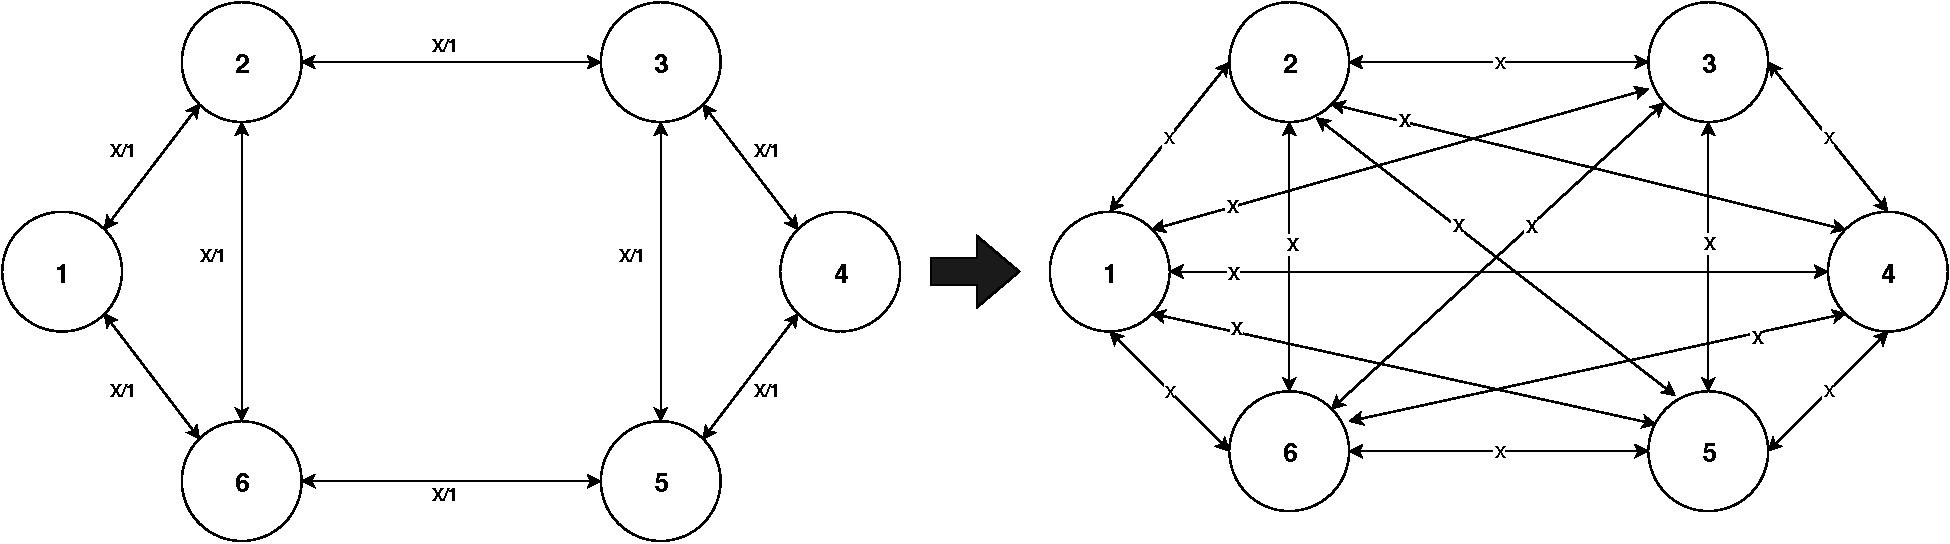
\includegraphics[width=1 \textwidth]{fig/logos/LogicalTopologyAlgorithm.pdf}
    \caption{Logical topology algorithm: conversion from physical topology (left side) to the logical topology (right side) for transparent transport mode.}
  \end{center}
  \label{logicalAlgorithm}
\end{figure}


\section{Routing}
\label{routing2}

Routing is the process of assigning a unique path through the network for a demand request between the source and destination nodes \cite{SimmonsJane2008}. %The number of paths generated can vary according to the user preference and so can the chosen key factor of Dijkstra's algorithm. Some examples to be considered are the number of links in the path, i.e., the number of hops, the distance of each path or the probability of the links being available. In this last case the metric is unrelated to distance and as such the term 'shortest paths' may in some cases be a misnomer \cite{SimmonsJane2008}. 
The first step to take into account when a demand is received by the network is to search in the logical topology manager block for a prior existent path between the same source/destination combination with remaining available capacity to route this demand. If there is any path with the characteristics described above then the same is re utilized to forward the demand, having no need to communicate with the physical topology manager block. In this case only the remaining capacity of the path needs to be updated. If on the other hand, there is no desirable path then a new one must be created to answer this demand request and if there is no possible way of establishing a new path then the demand request is blocked by the network. Below in sections \ref{candidate} and \ref{selecting} the steps taken to create and test a path for a demand are analysed in more detail.
\vspace{11pt}
\begin{figure}[H]
  \begin{center}
    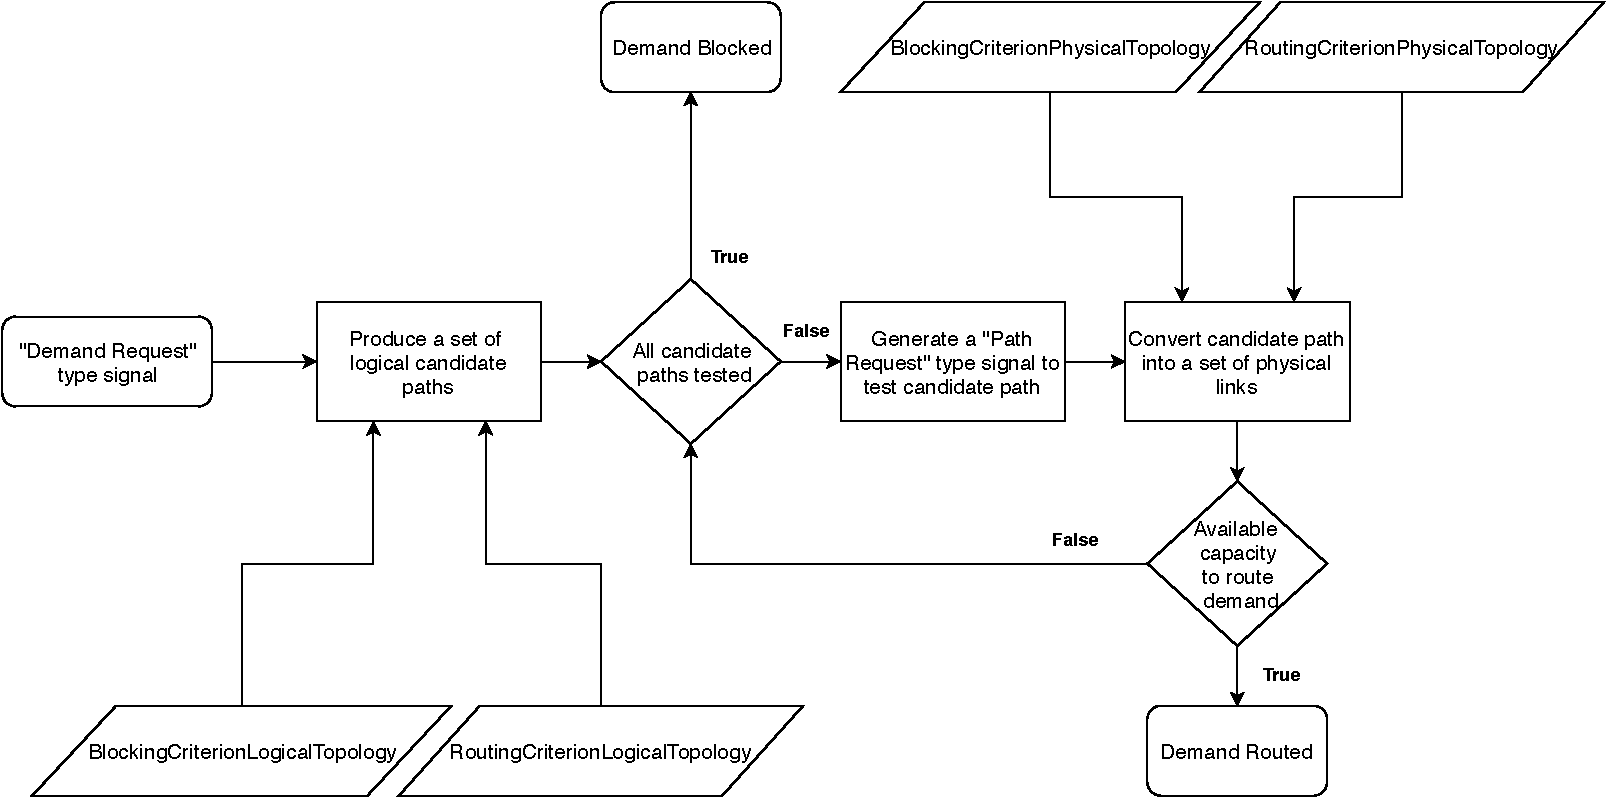
\includegraphics[width=1 \textwidth]{fig/logos/routing.pdf}
    \caption{Routing algorithm code flow.}
  \end{center}
  \label{routingAlgorithm}
\end{figure}

\subsection{Producing a set of candidate paths}
\label{candidate}

The routing strategy applied incorporates the use of a K-shortest path algorithm, based on Dijkstra's algorithm, in order to find the K-shortest paths between a source and a destination node \cite{SimmonsJane2008}. The number of paths generated both on the physical and logical layers will depend directly on the user preference. In transparent networks, where optical bypass is enabled, the need for optical regeneration favors in a way the use of distance as a metric to select the shortest paths. However, in this systems there is another major constraint to be considered which is the need for wavelength continuity, which means that a signal travelling from a source to a destination node must remain in the same wavelength as it optically bypasses intermediate nodes \cite{SimmonsJane2008}. Thus, arises another problem, finding a common available wavelength in all the constituting links of a path. The difficulty and complexity of achieving this escalates significantly as the number of links in the path increases as it shall be analysed further in section \ref{WA}. As such, it was decided to use the number of hops as the metric to find the shortest paths in the studies conducted. Other concerns, such as, considering a bottleneck-avoidance strategy in the routing stage to generate shortest paths with good link diversity  could have been taken into account if not for simplicity reasons.  

% FUTURE DIRECTION: Consider a bottleneck-avoindance strategy in the routing stage to generate shortest paths with good link diversity.



\subsection{Selecting a candidate path}
\label{selecting}

In this step it was used a dynamic-path routing strategy to the detriment of other strategies such as fixed or alternative-path routing, once it provides adaptability to network conditions \cite{SimmonsJane2008}. There is no prior determination of the paths to be used for a demand request between a given source and destination nodes. That calculation is performed when a demand request is received and it depends only of the current logical and physical topology states of the network. In the case a given logical or physical links have insufficient capacity to carry the new demand they should be momentarily withdrawn from the network topology so that in further iterations new demand requests that require the same capacity (same ODU type) don't consider those links while generating the set of candidate paths. After the topology has been trimmed based on the current network state the K-shortest paths algorithm can be applied \cite{SimmonsJane2008}.

\section{Grooming}
\label{G}

As the majority of the traffic going through the network usually requires a minor bit-rate than of a full wavelength, i.e., line-rate traffic, a necessity arose for a process capable of diminishing the percentage of wasted wavelength capacity, making networks more efficient \cite{SimmonsJane2008}. This process is named grooming, which is a simple way of grouping sub-rate traffic in order to better utilize networks capacity. In transparent networks the type of grooming performed is called end-to-end multiplexing, where traffic demands are packed into wavelengths and processed as a single unit from source to destination \cite{SimmonsJane2008}. In this transport mode demands may only ride together if the pair of source and destination nodes is the same.

\begin{figure}[H]
  \begin{center}
    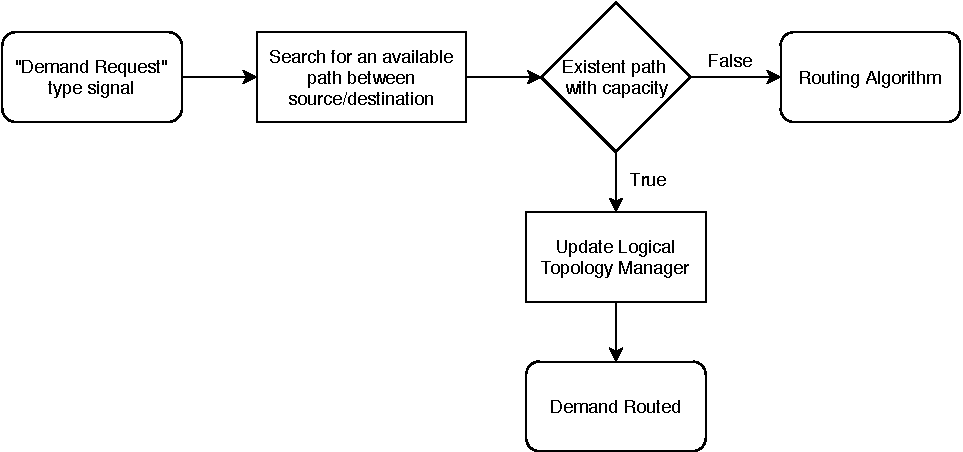
\includegraphics[width=0.9 \textwidth]{fig/logos/groomingAlgorithm.pdf}
    \caption{Grooming algorithm code flow.}
  \end{center}
  \label{groomingAlgorithm}
\end{figure}
\clearpage
In the framework discussed in chapter \ref{chapter3} the grooming stage occurs in the logical topology manager, where a demand being processed looks for an available path between the same pair of source and destination nodes, previously established and still with sufficient remaining capacity. If such a path exists than it will be re-utilized in order to route this demand and its capacity is refreshed but if not than the routing algorithm must be applied.

\section{Wavelength Assignment}
\label{WA}

\begin{figure}[H]
  \begin{center}
    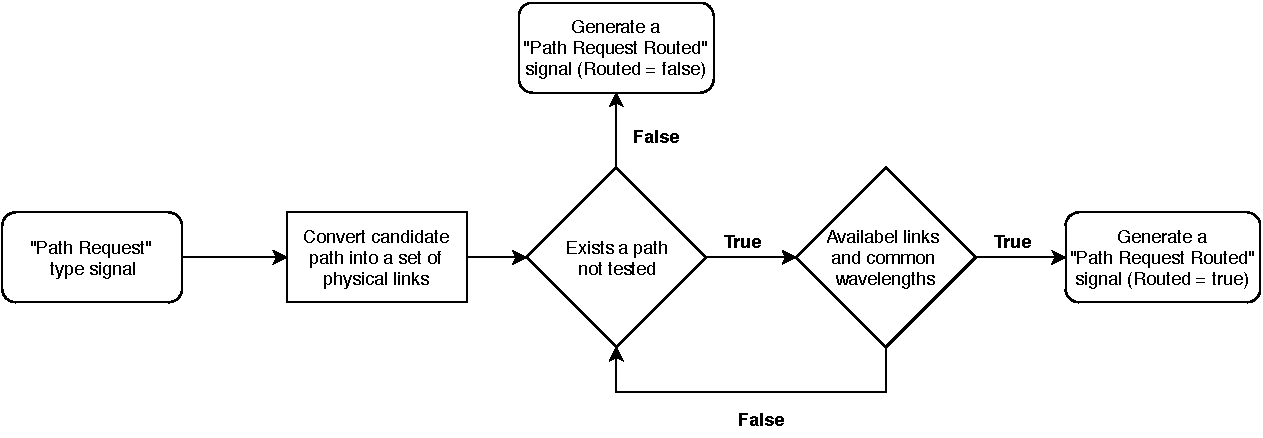
\includegraphics[width=1 \textwidth]{fig/logos/wavelengthAssignment.pdf}
    \caption{Wavelength Assignment algorithm code flow.}
  \end{center}
\end{figure}

This is one crucial step in transparent networks planning once they require wavelength continuity in all nodes from source to the destination, meaning that signals entering a source node are kept in the optical domain at every intermediate nodes of the path until reaching its destination \cite{SimmonsJane2008}. \gls{o-e-o} conversions are only performed in end nodes, therefore, the wavelengths that are in use in a particular link may have influence on the wavelengths that can be assigned to other links. This step follows the routing process. Thus, wavelength assignment is a major issue in optical-bypass networks once a poor routing strategy can lead to a situation of wavelength contention provoking the loss of network efficiency as demands are blocked instead of being routed. Another relevant aspect is how to choose the wavelength to assign to a certain connection from the set of all wavelengths supported on a fiber. The strategy adopted in this dissertation is commonly know as First-Fit\cite{SimmonsJane2008}, but other methods could also be applied, such as:
\begin{itemize}
  \item Most-Used.
  \item Relative Capacity Loss.
  \item Qualitative Comparison.
\end{itemize}
First-Fit was chosen for being the simplest of all these wavelength assignment schemes mentioned. Every wavelength has an associated index and the one with the lowest index is selected from the set of the available wavelengths. This strategy does not require global knowledge about the network and as the computational overhead is small and the complexity low the performance in terms of wavelength contention is among the best \cite{fisrtFit}.

\section{Chapter summary}

Many heuristic algorithms were implemented and tested along this dissertation. Starting by the scheduling algorithm, a very simplistic and straightforward strategy was implemented based only on the traffic quantity of each individual demand request. Although it has some advantages, like the minimum computational effort and time efficiency, it won't provide the best solutions for every practical scenario. In terms of routing, a dynamic-path routing strategy incorporating a K-shortest path algorithm was chosen once it provides adaptability to network conditions, which allows the avoidance of heavily loaded links, thus, lowering the blocking probability of the network. As the only the transparent transport mode was addressed the choice of the grooming strategy was bounded to an end-to-end single hop scheme. Finally, regarding the wavelength assignment process a first-fit strategy was adopted for its simplicity, low computational complexity and proper performance.


\cleardoublepage



